\documentclass{beamer}

\usepackage[utf8]{inputenc}
\usepackage{hyperref}
\usepackage{times}
\usepackage{graphicx}
\usepackage[ngerman]{babel}
%\usepackage[onehalfspacing]{setspace}
\usepackage{amsmath}
\setbeamertemplate{section in toc}[sections numbered]
\setbeamertemplate{subsection in toc}[subsections numbered]
\usepackage{bm}
\usepackage{multicol}


%Information to be included in the title page:
\title{Guided Quantum Diffuison Monte Carlo for Calculating Zero Point Energies}
\author{Simon Neidhart}
%\institute{Department of Physics, University of Basel}
\date{\today}


\begin{document}
\frame{\titlepage}

\section{Einleitung}
\begin{frame}
\frametitle{Was ist Monte Carlo?}
\begin{center}
Berechnung der Kreiszahl $\pi$ mit Zufallszahlen.
\scalebox{0.5}{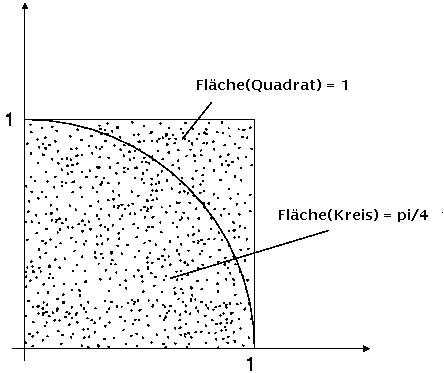
\includegraphics{pi.png}}\\ 
$\frac{\pi}{4} = \frac{N_{Kreis}}{N_{Quadrat}}$
\end{center}
\end{frame}

\section{Einleitung}
\begin{frame}
\frametitle{Quantenmechanik}
\begin{center}
Schrödingers Katze\\
\smallskip
\scalebox{1}{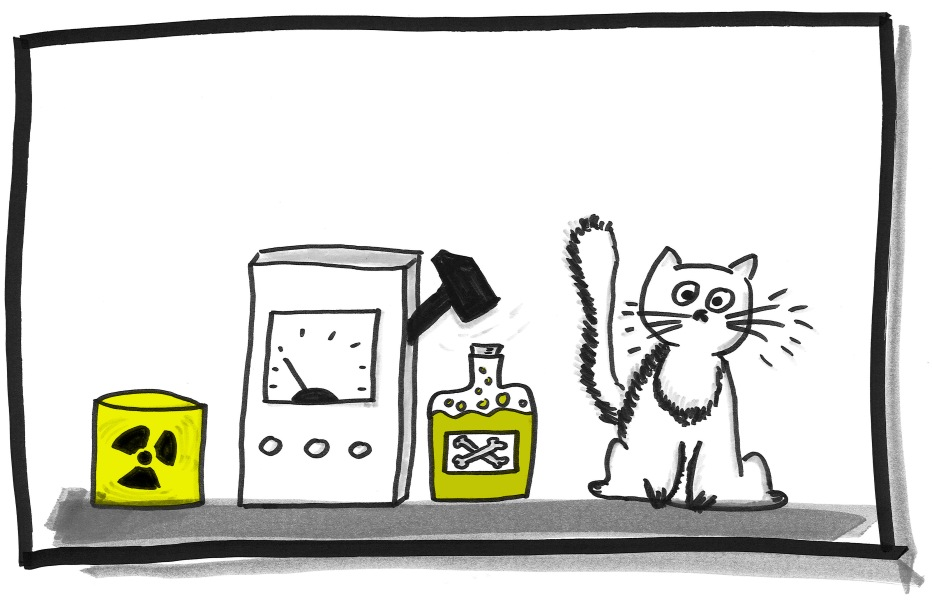
\includegraphics{cat.jpg}}\\ 
\end{center}
\end{frame}

\section{Einleitung}
\begin{frame}
\frametitle{Quantenmechanik}
\begin{center}
Heisenbergsche Unschärferelation\\
\medskip
\scalebox{1}{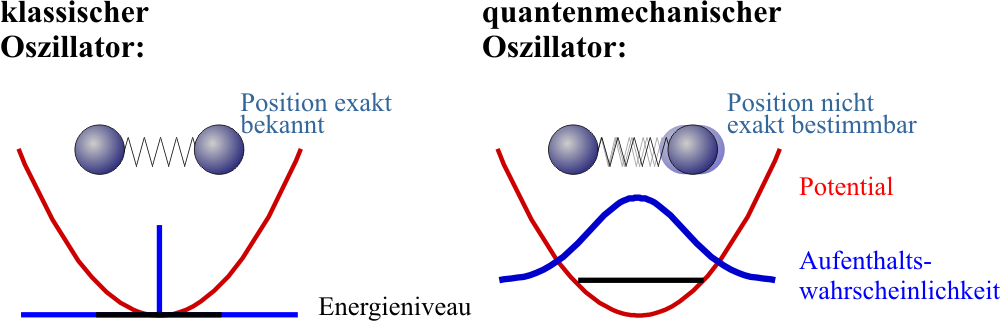
\includegraphics{harmonic.png}}\\ 

\smallskip
\end{center}
\begin{itemize}
\item Position und Impuls eines Teilchens können nicht gleichzeitig beliebig genau bestimmt sein.
\item Ziel: Berechnen des Energieunterschiedes klassischer/quantenmechanischer Oszillator (zero point energy).
\end{itemize}
\end{frame}

\section{Einleitung}
\begin{frame}
\frametitle{Der DQMC Algorithmus}
\begin{itemize}
\item Lösen der Schrödinger Gleichung (hochdimensionale Differentialgleichung) mit Monte Carlo.
\item Benutzen des harmonischen Oszillators zum berechnen einer "guiding"  Wellenfunktion.
\end{itemize}
\begin{center}
\scalebox{0.5}{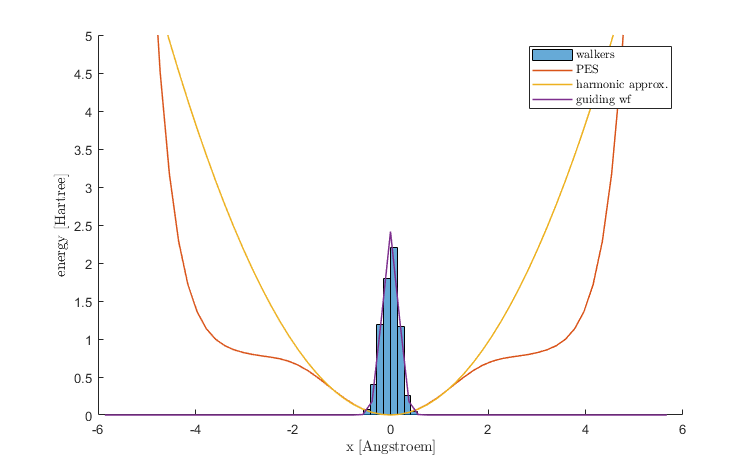
\includegraphics{guiding.png}}\\ 
\end{center}
\end{frame}

\section{The DQMC Algorithm}
\begin{frame}
\frametitle{Untersuchte Systeme}
\begin{multicols}{2}
    \begin{center}
    Ethan ($C_2 H_6$)\\
	\scalebox{0.08}{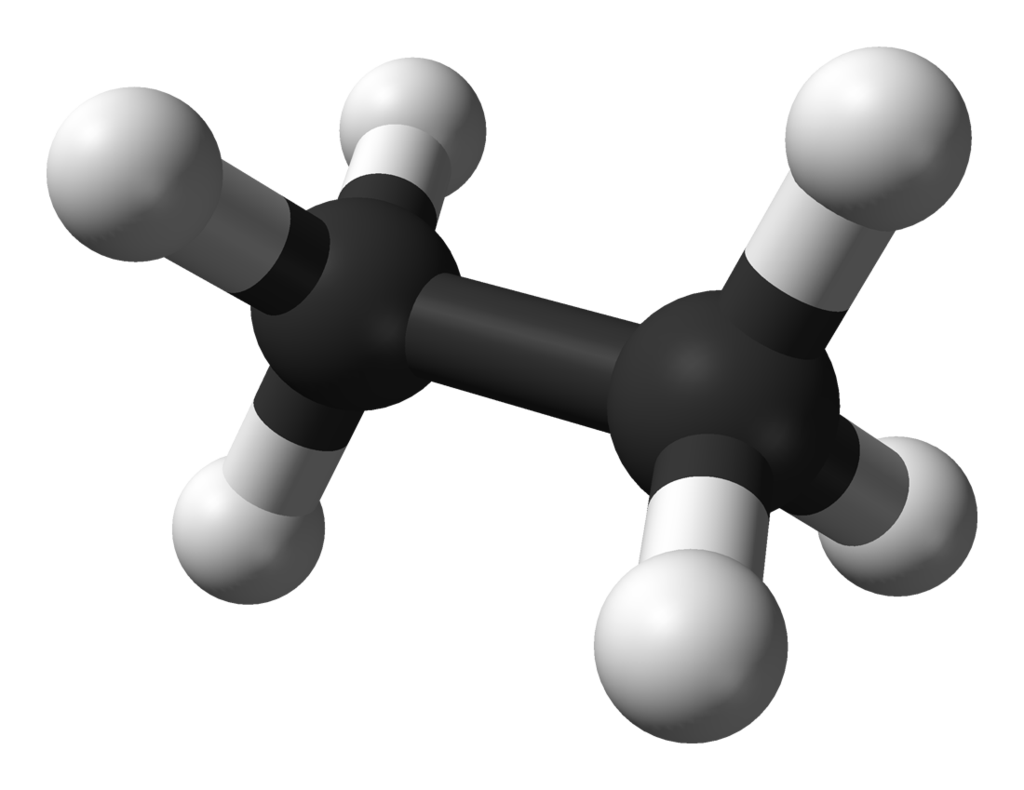
\includegraphics{p1.png}}\\
	2-Phenylphenol ($C_{12} H_{10} O$)\\
	\scalebox{0.15}{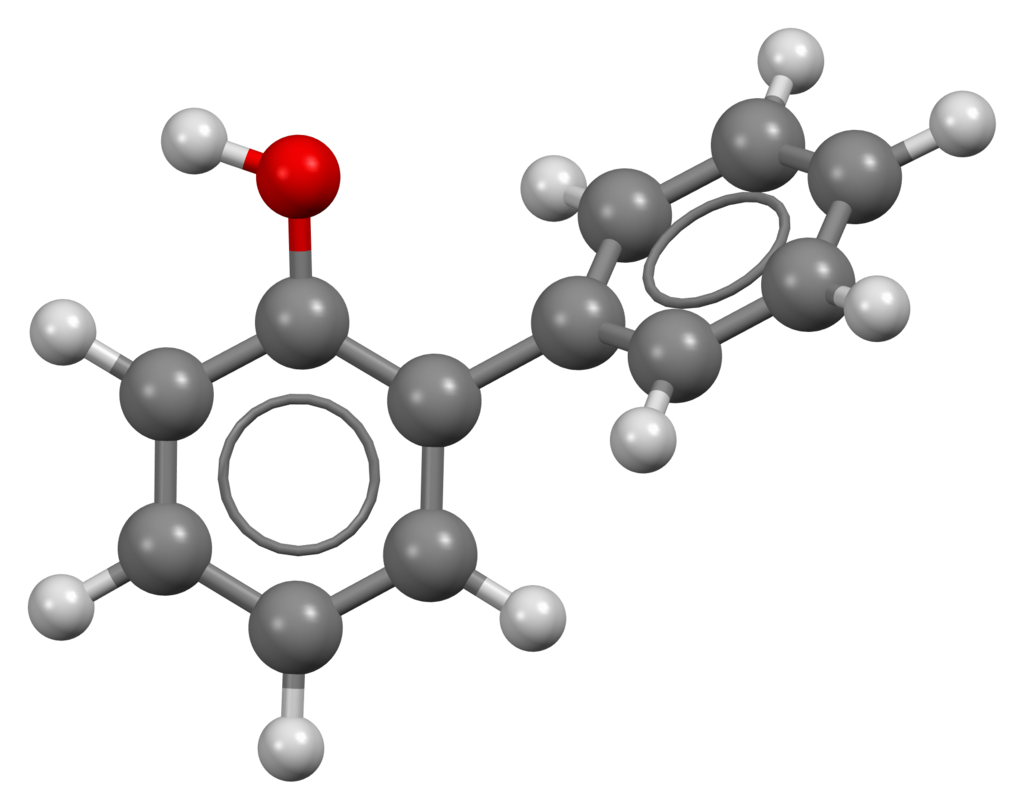
\includegraphics{p2.png}}\\
	Endohedrale Komplexe\\
	(z.B. $H_2@C_{60}$)\\
	\scalebox{0.15}{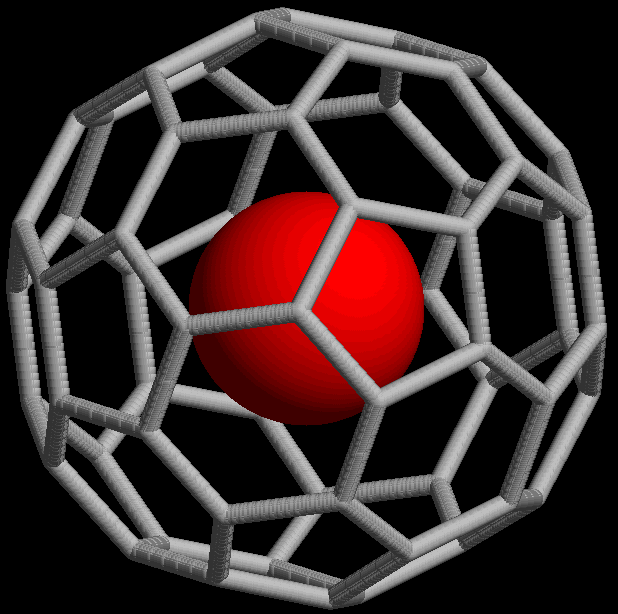
\includegraphics{p3.png}}\\
	\end{center}
\end{multicols}
\end{frame}

\begin{frame}
\frametitle{Resultate}
\begin{center}
\scalebox{0.35}{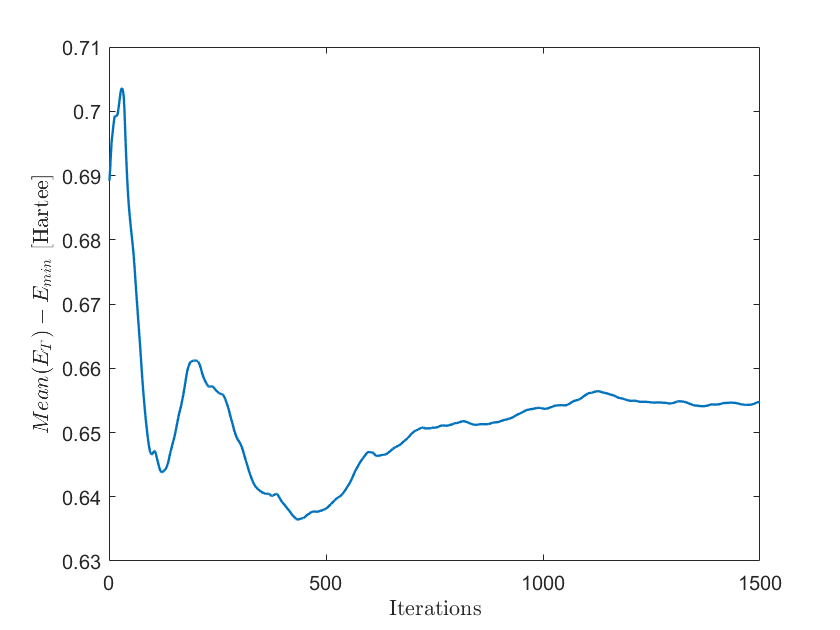
\includegraphics{results.png}}\\ 
Konvergenz der zero point Energie von $H_2@C_{60}$.
\end{center}
\end{frame}

\section{Einleitung}
\begin{frame}
\frametitle{Weitere Anwendungen von Monte Carlo}
\begin{itemize}
\item Allgemein: Berechnung von hochdimensionalen Integralen
\item Wettervorhersage/Klimasimulationen
\item Vorhersagen bei der Produktion von Windenergie
\item Umgebungserkennung von Robotern mit Kamera
\item Bewertung von Investment-Projekten
\item Vermutlich auch Stabilitätsanalysen von Stromnetzen. 
\end{itemize}
\end{frame}

\end{document}